\documentclass[12pt]{article}

\usepackage{color,graphicx,overpic}
\usepackage[margin=1.0in]{geometry}

\begin{document}
\noindent\textsc{\large CS 314 Final Review --- Reverse Doubly Linked List}

\vspace{6pt}
\noindent\textbf{Linked Lists}

\vspace{2pt}
\noindent  Write an instance method for a doubly linked list which reverses the order of the elements in the list. The first element will 
become the last element, the second becomes the second-to-last, etc. 

\vspace{2pt}
\noindent The doubly linked list class provided, \texttt{DoubleLinkedList}, has doubly linked nodes and the list is null terminated at both ends.
There are no special header nodes, all nodes contain elements of the list. The following is a visual digram of this list class:

% List diagram
\begin{figure}[h!]
  \hfill
  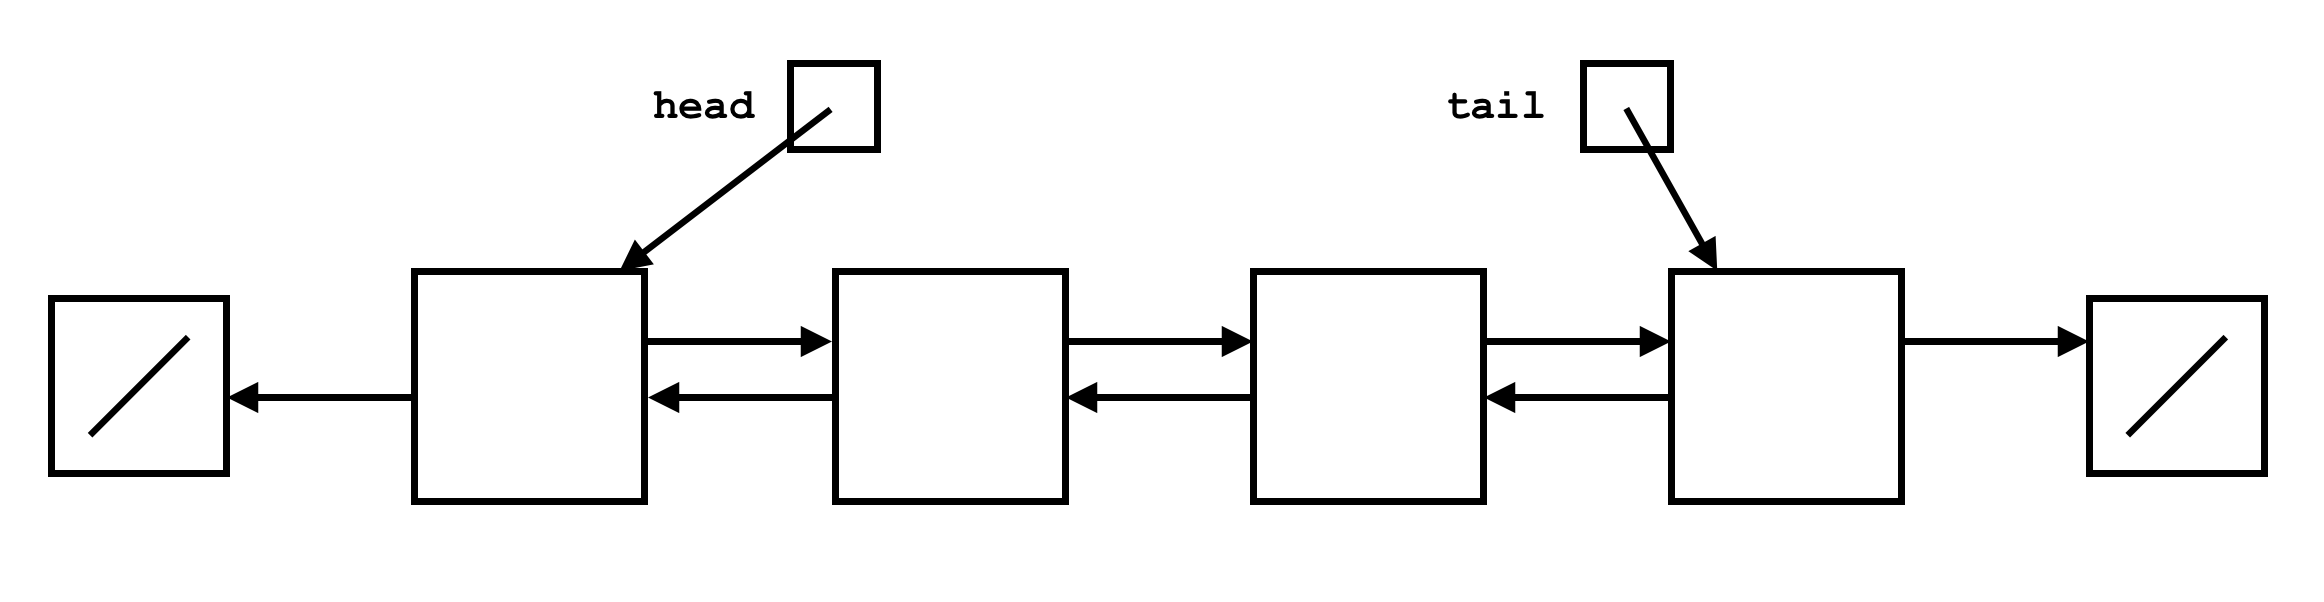
\includegraphics[width=115mm, scale=0.5]{diagram.png}
  \hspace*{\fill}
\end{figure}

\noindent Examples of calls to \texttt{reverseList()}. The result shown is the new state of \texttt{this}.
\begin{itemize}
  \item \texttt{[0, 1, 2, 3].reverseList() => [3, 2, 1, 0]}
  \item \texttt{[3, 1, 4].reverseList() => [4, 1, 3]}
  \item \texttt{[5, 5, 5].reverseList() => [5, 5, 5]}
  \item \texttt{[7].reverseList => [7}
  \item \texttt{[].reverseList => [}
\end{itemize}

\vspace{6pt}
\noindent Use the follwing \texttt{DoubleLinkedList} implementation.
\begin{verbatim}
public class DoubleLinkedList<E>{

   

  private static class DoubleListNode<E>{
    DoubleListNode<E> prev, next;
    E data;
  }
}
\end{verbatim}

\noindent You may create new \texttt{DigitNode} objects using the provided constructor.

\noindent \textbf{You may not create any other data structures.}

\noindent Do not use any other Java classes or methods.

\clearpage
\begin{verbatim}
/* Pre:  val >= 0; this list is in a valid state -> first != null
 * Post: this list will represent the sum of the previous state + val
 *       this list will still be in a valid state
 */
 public void addValue(int val){
\end{verbatim}
\end{document}
